\documentclass[12pt]{article}

\usepackage{fullpage}
\usepackage{graphicx, rotating, booktabs} 
\usepackage{times} 
\usepackage{natbib} 
\usepackage{indentfirst} 
\usepackage{setspace}
\usepackage{grffile} 
\usepackage{hyperref}
\usepackage{adjustbox}
\usepackage{amsmath}
 \usepackage{multirow} 
\setcitestyle{aysep{}}


\singlespace
\title{\textbf{Alliance Participation, Treaty Depth, and Military Spending}}
\author{Joshua Alley\footnote{Postdoctoral Research Associate, University of Virginia.}}
\date{}

\bibliographystyle{apsr}

\begin{document}

\maketitle 

\doublespace 

\begin{abstract}
How does alliance participation affect military spending? 
Some argue that alliance membership increases military expenditures, while others contend that it produces spending cuts.
I argue that deep formal defense cooperation modifies the impact of alliance participation on military expenditures.  
When security-seeking non-major powers join deep alliances they usually decrease military spending, because these treaties are more credible.
Joining shallow alliances often increases non-major power military spending, however.    
I test the argument by creating a latent measure of alliance treaty depth and using it to predict differences in how alliance participation affects military spending. 
The research design generates new empirical evidence linking alliance participation and percentage changes in state military spending from 1816 to 2007. 
I find that deeper alliance treaties tend to decrease non-major power military spending, and shallow alliances often increase military spending.  
These results help scholars and policymakers better understand a central question about alliance politics that has been debated in scholarship for decades. 
\end{abstract}


\newpage 


\section{Introduction}


Scholars of international relations have long acknowledged that there are two ways for states to increase their security. 
They can invest in indigenous military capability or form alliances \citep{Morgenthau1948, Altfield1984, Morrow1993}.
Because both policies provide security, broadly defined, alliance participation should change how states invest in military capability. 
But exactly how alliances influence military spending remains unclear. 


Existing scholarship contains contradictory theoretical predictions and evidence on the question of alliance participation and military spending. 
One view expects that alliance participation will reduce military spending e.g., \citep{BarnettLevy1991, Morrow1993, Conybeare1994}. 
The other predicts that alliance participants will spend more on defense e.g., \citep{Diehl1994, MorganPalmer2006, QuirozFlores2011}.
This paper addresses the divide by using alliance treaty design to explain when alliance participation leads to more or less defense spending. 
In doing so, it helps clarify a longstanding debate about alliance politics.


I use variation in alliance design and membership to predict how alliance participation affects military spending. 
Scholars have engaged in extensive study of the sources and consequences of differences in alliance treaty design and membership \citep{Mattes2012, Benson2012, Poast2019a, Morrow1991, Leeds2003, LeedsAnac2005, Fordham2010, Mattes2012,  Poast2013, Johnsonetal2015}. 
Despite the importance of different alliance treaty designs for outcomes like conflict \citep{Leeds2003, Benson2012} and trade \citep{Long2003, LongLeeds2006} the debate about alliance participation and military spending has largely treated alliances as homogeneous.\footnote{See \citet{DigiuseppePoast2016} for an important exception.}
But alliance participation could plausibly increase or decrease defense expenditures, under different alliance treaties. 
In particular, I emphasize how treaty depth modifies the impact of alliance participation on military spending. 
Deep alliances formalize extensive defense cooperation between members. 
In addition to commitments of military support, deep treaties require defense coordination and cooperation among alliance members. 


To explore the consequences of deep and shallow alliances, I examine a particular set of states: non-major powers. 
I focus on non-major powers because these states clearly show a tradeoff between reassurance and allied military spending in deep alliances.
Participation in deep alliances allows non-major powers to reduce military spending due to greater treaty credibility and reduced allied leverage on defense spending. 
Joining a shallow alliance often increases non-major power military spending because realizing foreign policy gains from alliance participation depends on defense spending when members fear abandonment.

 
I employ a novel research design to test my argument.
First, I develop a latent measure of alliance treaty depth. 
I then incorporate that measure into a multilevel model which estimates how alliance characteristics modify the impact of total allied defense expenditures on annual percentage changes in military spending.
Because allied capability is the ultimate source of security in alliances, I use total allied capability to measure alliance participation.  
Allied capability is a useful proxy for alliance participation because it combines the impact of joining an alliance and changing allied capability during treaty membership, both of which change the security benefits of alliance participation. 
Multilevel modeling matches my conditional argument and captures heterogeneous effects of alliance participation across individual treaties. 
I fit the model on a sample of non-major power states from 1816 to 2007 and find that while deep alliances decrease percentage changes in non-major power military spending, participation in shallow alliances often increases spending.


The argument and findings illuminate a salient debate in US foreign policy about the costs and benefits of alliances. 
Advocates of deep engagement \citep{Brooksetal2013} and restraint \citep{Posen2014} in grand strategy have different views of alliances. 
Proponents of restraint argue that the United States should withdraw from many alliances, because allies spend too little on defense, which then increases US defense spending \citep{Preble2009}.
The deep engagement school argues that the benefits of alliances exceed the costs and believe that the problem of low allied military spending is overstated \citep{BrandsFeaver2017}. 
My argument and findings suggest that policymakers can adjust alliance commitments to reassure partners or encourage higher allied military spending, but will struggle to do both. 
The United States often uses deep alliances to reassure partners, but this may encourage lower allied military spending. 
This tradeoff suggests that there is little room for compromise between deep engagement and restraint in grand strategy.  


The paper proceeds as follows. 
First, I summarize competing claims on alliance participation and military spending. 
Then I describe my argument in more detail. 
After the argument, I present the research design and results. 
The final section concludes with a discussion of the results and implications for scholarship and policy.  



\section{Do Alliances Increase or Decrease Military Spending?}


% quick intro and straight into it
Scholarship on alliance participation and military spending is divided between two views.
One expects that alliance participation will decrease military spending, while the other anticipates a positive relationship between alliance participation and defense expenditures. 
Each view predicts a different average effect of alliance participation by emphasizing one aspect of alliance politics.   


Two types of arguments predict a negative association between alliance participation and defense spending. 
First, the economic theory of alliances \citep{OlsonZeckhauser1966} claims that alliances are subject to a collective action problem because security from an alliance is a public good.
Because alliance security is neither rivalrous nor excludable, members contribute inadequate resources to collective defense. 
Alliance members can ``free-ride'' and smaller states exploit larger partners. 
Lower spending allows alliance members to consume more non-defense goods, but the alliance provides suboptimal security.\footnote{\citet{SandlerForbes1980}, \citet{Oneal1990} and \citet{SandlerHartley2001} all modify the public goods logic while relying on Olson and Zeckhauser's core intuition.} 
Second, substitution arguments recognize that states employ one policy in place of another \citep{MostStarr1989}.
Alliances provide security without requiring additional military spending \citep{Morrow1993, Conybeare1994}. 
Given extra security, states rely on their allies and and reallocate military spending to other goods. 
Both the substitution and public goods models expect that alliance participation reduces military spending due to the opportunity costs of military expenditures. 
States want to rely on their allies for security because higher defense expenditures leave fewer resources for other goods \citep{Fordham1998, Fearon2018}.


A contradictory perspective asserts that alliance participation increases military expenditures. 
Several arguments predict higher military spending by alliance members, using a shared intuition that states increase military spending to support their alliance commitments. 
\citet{Diehl1994} argues that alliances create new foreign policy obligations, necessitating extra military spending.
Because alliances expand what a state can achieve in international relations, states might increase military spending to pursue other foreign policy goals \citep{MorganPalmer2006}.
For example, buffer states use conscription to make themselves a more attractive alliance partner \citep{Horowitzetal2017}.
Others assert that cooperation within alliances generates higher defense spending \citep{Palmer1990, QuirozFlores2011}. 
These predictions of a positive correlation between alliance participation and military spending contradict expectations of lower military spending by alliance members.\footnote{
\citet{SeneseVasquez2008} argue that military spending and alliances are part of a conflict spiral of simultaneous growth in military expenditures and alliance participation, which suggests that conflict behavior drives any correlation between alliances and military spending. 
}


\subsection{Mixed Evidence} 


Mixed findings reinforce theoretical divisions between the contradictory views of alliances.
Some studies find a positive association between alliance participation and military spending. 
Others find a negative relationship.\footnote{
Because tests of the public goods model use military spending as a share of GDP as the their outcome of interest, I do not include most of those results in this summary.} 


% Specific and general studies
Scholars have studied the connection between alliance participation and military spending in two ways. 
General studies of military spending and alliances compare many states through dummy indicators of alliance participation, which collapse alliances into a state-level measure. 
This design compares states with at least one alliance to those with none.
By contrast, specific research designs examine defense expenditures within a single alliance. 
Much of this work seeks to explain variation in spending among NATO members, focusing on how states respond to increases in contributions to collective defense by the United States.


\autoref{tab:results-sum} summarizes previous results on the issue of alliance participation and military spending. 
Both specific and general research designs produce mixed findings. 
There is one negative, three positive and two null estimates of the correlation between alliance participation and spending in general studies. 
Specific studies turn up five negative and two positive results.  


\begin{table}[hbt!]
\begin{center}
\begin{tabular}{lcccc}
   Research Design  & Study & Decrease & Increase & Null \\
\hline
\multirow{5}{*}{General} & \citet{MostSiverson1987} &  &  & X \\
 & \citet{Conybeare1994}    & X & &  \\
 & \citet{Diehl1994}        &  & X &  \\
 & \citet{Goldsmith2003}    &  &  & X \\
 & \citet{MorganPalmer2006} &  & X & \\ 
 & \citet{QuirozFlores2011} &  & X &  \\ 
 \hline
 \multirow{7}{*}{Specific} &\citet{ConybeareSandler1990} &   & X &  \\
 &\citet{BarnettLevy1991} & X  &  &  \\
 &\citet{Morrow1993}      & X  &  &  \\
 &\citet{Sorokin1994}     & X  &  &  \\
 &\citet{Chenetal1996}    &  & X &  \\
 &\citet{PluemperNeumayer2015} & X &  &  \\
 &\citet{GeorgeSandler2017} & X &  &  \\
\hline
\end{tabular}
\caption{Findings of the association between alliance participation and military spending. The top block details results from general studies, which compare states with at least one alliance to states without any alliances. The bottom block shows results from specific studies, which examine how national military spending changes in response to shifting allied capability.}
\label{tab:results-sum}
\end{center} 
\end{table}


The mixed empirical results reflect a theoretical problem. 
Both perspectives make unconditional claims about the average effect of alliance participation on military spending.  
With one exception \citep{DigiuseppePoast2016}, scholarship on alliance participation and military spending ignores differences between alliances.
Treaty obligations and membership vary widely across alliances, however \citep{Leedsetal2002}. 
I focus on a key difference between alliances that can help us understand their heterogeneous effects on military spending: the depth of military cooperation in the treaty.



\section{Argument}

% outline the whole argument
My argument explores how deep military cooperation in an alliance treaty modifies the impact of alliance participation on non-major power military spending.
Because non-major powers focus on security, alliances protect them from external threats. 
Treaty depth shapes whether the security benefits of alliance participation depend on military spending. 
Even in the face of significant threats, non-major powers can gain more security with less military spending if they form deep alliances. 
Conversely, security gains in shallow alliances often depend on non-major powers maintaining or even increasing their military spending to manage abandonment concerns. 


% justify non-major power emphasis
I focus on non-major powers to maintain theoretical and empirical parsimony.
As I explain below, major and non-major powers use alliances to achieve different foreign policy goals, which changes how alliance participation affects their military spending. 
My argument also provides novel insights about non-major powers.  
Some scholarship and much popular discourse assumes that non-major powers regularly reduce military spending in alliances.
I challenge this assertion by showing that alliance participation sometimes requires non-major powers to increase defense expenditures. 


% Summarize the flow of the argument
I start the argument by describing a general framework where alliances are institutionalized military cooperation between states. 
Then I discuss how deep formal military cooperation affects alliance credibility. 
Last, I explain how alliance depth affects the connection between alliance participation and non-major power military spending. 


\subsection{Cooperation in Alliances}

% opportunistic behavior in alliances and international cooperation 
Alliances are a form of international cooperation. 
Promising military support through a treaty generates a credible commitment of intervention \citep{Fearon1997, Morrow2000}. 
Allied support then helps members achieve crucial foreign policy goals like deterrence or winning wars \citep{Walt1990, Snyder1997}. 
States form alliances so they can use other states' military capabilities to back their foreign policy aims.


Because allied capability gives a treaty foreign policy value, alliance participation is inseparable from allied capability \citep{FordhamPoast2014}. 
The presence of an alliance treaty formalizes when a state can expect military intervention \citep{Morrow2000}, but the treaty itself does not provide security. 
Allied capability is the ultimate source of security in an alliance. 
Greater allied capability increases the value of an alliance, all else equal \citep{Johnsonetal2015}, so I conceptualize alliance participation in terms of allied capability.\footnote{A binary conceptualization of alliance participation assumes all alliances are equally valuable.}


% Alliance formation models and focus on non-major powers.  
Alliance treaties and the capability they draw on can support many foreign policy aims, which often facilitates exchanges between alliance participants. 
One common exchange occurs in asymmetric alliances between major and non-major powers \citep{Morrow1991}. 
Large states form asymmetric alliances to increase their foreign policy influence, while smaller partners gain protection from external threats. 
Not all alliances are asymmetric,\footnote{130 of 289 ATOP alliances with offensive or defensive obligations are asymmetric pacts with at least one major and one non-major power, but a further 122 alliances are symmetric treaties between non-major powers.} but the divergent motives of major and non-major powers in these treaties reflect general tendencies in alliance politics. 
Major powers often use alliances to address the global balance of power and increase their influence. 
Smaller non-major powers tend to emphasize immediate security and regional concerns in their alliances. 
As a result, there are distinct processes behind non-major and major power alliance participation and these states respond to allied capability and treaty design in different ways. 


% Can think about this as an enforcement problem: non-major powers fear abandonment
Non-major powers use allied support to provide protection from external threats. 
But as with all cooperation, alliance members must account for opportunism, or ``behavior with guile'' \citep{Williamson1985}. 
Even as states commit to an alliance, they can also benefit from defecting and taking advantage of allied cooperation. 
Sometimes the perceived benefits of defection outweigh the long-run benefits of cooperation, so alliance members face an enforcement problem \citep{Fearon1998a, Koremenosetal2001}.


% Problem of abandonment
Non-major powers are especially concerned with abandonment, which is the most common form of opportunism in alliances.
One estimate suggests that the rate of compliance with military intervention obligations is only 50\% \citep{BerkemeierFuhrmann2018}.
For security-focused non-major powers, these alliance violations threaten their main goal. 
Concern with abandonment then affects military spending decisions. 


Abandonment and military spending are related because greater alliance credibility allows states to lower military expenditures.\footnote{The public goods model of alliances calls reduced military spending in alliances free-riding. I do not use this language because it has come to imply that reduced defense spending is problematic. But as \citet[pg. 278]{OlsonZeckhauser1966} themselves observe, lower defense spending is not normatively problematic.}
Though states can augment the collective military capability of an alliance through investing in military capability, they can also reduce defense spending and rely on their partners \citep{OlsonZeckhauser1966, Morrow1993, Conybeare1994, SandlerHartley2001}.
Under credible alliances, such reductions in military expenditures are more likely, because states have less fear of abandonment. 


As \citet{DigiuseppePoast2016} observe, some alliances have fewer credibility concerns due to members' political regime type.
They show that defense pacts with democracies lower defense spending, as democracies make more credible commitments.
This insight about conditional credibility is a useful starting point because credibility is multifaceted. 
In treaty design, depth, unconditional military support \citep{Benson2012, Chibaetal2015} and issue linkages \citep{LongLeeds2006, Poast2012, Poast2013} all increase credibility.\footnote{Though the argument emphasizes depth, the research design accounts for multiple sources of alliance credibility.}
In this paper, I focus on treaty depth, which is a costly promise that allows alliance members and potential adversaries to infer the credibility of the alliance \citep{Leeds2003, FuhrmannSechser2014}. 


% Allied preferences on military spending
If alliance participation can reduce non-major power military spending, is that a problem for their allies? 
This argument assumes that allied states usually prefer higher non-major power military spending because it adds capability to the alliance.\footnote{This preference is somewhat attenuated by concern that substantial changes in capability will provide too much autonomy. For example, the United States has inhibited nuclear acquisition by some allies \citep{Gavin2015, Lanoszka2015}.}
Allies also encourage higher military spending so their partners can manage internal threats.
This preference for higher defense spending is not a driving force in alliance treaty design, however, because states prioritize abandonment and entrapment concerns in treaty design. 
States cannot form an alliance without addressing abandonment and entrapment, but they can leave bargaining over military spending to alliance maintenance \citep{Snyder1997}.
Also, some evidence suggests that alliance negotiations emphasize when and how states provide military support \citep{Poast2019a}. 


Assuming that allies of non-major powers usually prefer higher military spending is reasonable. 
States often sell or transfer weapons to allies in order to augment allied capability \citep{Yarhi-Miloetal2016, Pampetal2018}. 
Even in alliances between superpowers and non-major powers, where highly asymmetric capability and interests might reduce concerns about non-major power defense expenditures, superpowers often encourage higher military spending. 
US demands for higher military spending by NATO members are well-known \citep{SchuesslerShifrinson2019}.
The Soviet Union also regularly pressured Warsaw Pact members to increase defense spending \citep{Simon1985}. 


When allies want non-major powers to spend more, enforcing such cooperation is difficult. 
Normative appeals to common interests are ineffective. 
Though verbal communication or ``cheap talk'' has value in international politics \citep{Trager2010}, it is unlikely to overcome the opportunity costs of defense spending. 
Even after reducing defense expenditures, alliance members retain foreign policy benefits and can reallocate resources to other priorities. 
The ability to reduce defense spending and spend more on other goods sometimes motivates states to form alliances \citep{Kimball2010, AllenDigiuseppe2013}. 


% Need leverage 
Therefore, if alliance members want to encourage greater allied defense spending, they need leverage. 
States gain leverage either from a credible threat to abandon low-spending partners or direct control over allied policies. 
Policy control of allied spending decisions occurs when the alliance reflects hierarchical relationships \citep{Lake1996}. 
Without such direct influence, states must possess a credible threat to leave the alliance over low defense spending. 
Otherwise, allies will dismiss weaker signals and threats due to uncertainty and incomplete information. 


% adding credibility/reassuring reduces leverage
Reassuring allies reduces the credibility of threats to abandon states that spend too little on defense. 
States cannot simultaneously reassure their allies and maximize leverage on defense spending. 
As alliance members use costly commitments to reassure, partners have more freedom to reduce defense spending. 


% Talk about more credible alliances
Under less credible alliances, low military expenditures could increase the risk of abandonment, so members have less freedom to reduce defense spending. 
Moreover, although states in less credible alliances increase their foreign obligations, they also face the risk of having to meet foreign contingencies without allied support. 
As treaty credibility falls, the foreign policy benefits of alliance participation become contingent on military spending.\footnote{For example, \citep{NiouZeigler2019} use a formal model to show that in alliances between rivals, states are less likely to reduce military spending, because their foreign policy gains from alliance participation depend on military spending.} 
This occurs because alliance members must hedge against abandonment and partners can leverage that concern to encourage higher defense spending.
Thus, alliances with less credibility will be more likely to increase military spending. 


% Transition- depth of military cooperation shows this tradeoff 
Treaty depth highlights this tradeoff between reassurance and military spending.
Where deep alliances often reduce non-major power military spending, participation in shallow alliances often increases it. 
Stipulating deep cooperation reassures partners and reduces leverage over allied military expenditures. 
Credibility from treaty depth also promotes efficiency gains from coordinated defense effort. 
I now describe the role of treaty depth in more detail. 



\subsection{Alliance Treaty Depth} 


I focus on depth because it provides theoretical leverage to predict when alliance participation increases and decreases military spending, which reveals a trade off between reassurance and defense spending.  
Moreover, treaty depth is a common policy choice.\footnote{In a related paper, I explore the sources of alliance treaty depth. All the sources of depth that paper identifies are included as control variables in the empirical analysis. Average democracy and threat at the time of alliance formation are the two largest sources of higher treaty depth.} 
Though states probably do not change their political regime to reassure allies, they often form deep alliance treaties. 
Over half of defensive or offensive ATOP alliances have some depth. 


% Define depth again 
Alliance depth is the extent of defense cooperation formalized in the treaty. 
Deep alliances require additional policy coordination and military cooperation beyond a promise of military support. 
While shallow alliances stipulate more arms-length cooperation between members, deep treaties lead to closer cooperation. 
Defense cooperation in a deep alliance takes many forms. 
Allies can form an integrated military command, provide military aid, commit to a common defense policy, provide basing rights, set up an international organization or undertake companion military agreements. 
All of these obligations move alliance members away from an arms-length partnership towards close cooperation via policy coordination and regular interaction, while imposing monetary and policy autonomy costs.\footnote{Although depth can have monetary costs, reductions in military spending due to greater treaty credibility will often outweigh those costs. Alliance contributions are a small part of most defense budgets, and non-major powers rarely use basing rights in deep alliances to deploy their troops abroad.} 

 
One example of a deep alliance is a 1948 defense pact between the United Kingdom and Jordan.
This alliance included basing rights, military aid, official military contact, and an Anglo-Transjordan Joint Defense Board.  
The basing, aid, and cooperation added more depth than a 1912 treaty between Greece and Bulgaria which only commits to mutual defense and consultation if either state is attacked by Turkey. 


% Emphasis: credibility and efficiency for lower milex
Deep alliances like the Anglo-Jordanian pact reduce non-major power military spending in two ways. 
First, depth reassures partners and reduces leverage on defense spending.  
Deep alliances are more credible because defense cooperation is costly. 
Making costly commitments of bases, policy coordination, or aid reassures allies \citep{Morrow1994}. 
Depth is especially useful because alliance members face a time inconsistency problem. 
Alliance treaty fulfillment depends on shared foreign policy interests \citep{Morrow2000, Leeds2003a}, so changing foreign policy interests threaten alliance fulfillment \citep{LeedsSavun2007}. 
A deep alliance makes a series of repeated transfers, and states can signal commitment by maintaining those transfers.\footnote{Conversely, eliminating or reducing planned transfers reduces the credibility of the whole alliance.} 
Second, credibility in deep alliances can facilitate more efficient defense spending, as alliance members to provide specific capabilities. 
Specialization means members of deep alliances spend less on the military but retain adequate security.
These efficiency gains depend on the credibility of the alliance, because states will only specialize if they believe the alliance is reliable \citep{Leeds2003a}.  


On the other hand, shallow alliances are less credible, so participation in these treaties is more likely to increase military spending. 
Shallow alliances have some basic credibility from hands-tying signals \citep{Fearon1997}, as well as the audience \citep{Morrow2000} and reputational \citep{Gibler2008, Crescenzietal2012} costs of violation.
Even so, threats to abandon low-spending allies are more credible than in a deep alliance where partners have taken pains to reassure their partners.  
In a shallow alliance, members must hedge against abandonment, which partners can use as leverage to discourage low defense spending. 
Maintaining the benefits of alliance participation then requires defense spending, because low military spending might endanger the treaty or expose states to adverse consequences if they are abandoned. 
Shallow alliances are also less likely to facilitate military specialization due to the fear of abandonment. 
As a result, participation in shallow alliances often increases military spending.\footnote{
One objection to this argument is that deep alliances are more valuable to members, which augments allied influence on defense spending. 
Although alliance value adds some leverage, it cannot offset reducing the credibility of threats to abandon low-spending allies.
Value increases leverage because states fear their allies will abrogate a valuable alliance, and deep alliances counteract this essential concern. 
}


% Cases
To illustrate the logic, consider two related alliances from the inter-war period. 
A 1920 treaty between France and Belgium (ATOPID 2055) added commitments of military aid and policy coordination to defensive obligations. 
Given this depth, the Franco-Belgian alliance reduced Belgian defense expenditures, even while Belgium helped occupy the Ruhr. 
A more limited treaty with only military support between France, Belgium, the United Kingdom, Italy and Germany (ATOPID 2130) increased Belgian spending, on the other hand.   
 
 
Taken together, the examples and argument suggest that treaty depth modifies the impact of alliance participation on non-major power military spending. 
Shallow alliances often increase military spending, and deep alliances usually reduce spending.  
Therefore, with a continuous conceptualization of depth, there should be a negative correlation between treaty depth and the impact of alliance participation on non-major power military spending as the positive effects of shallow treaties turn into negative effects in deep alliances. 
This implies three separate hypotheses, one about shallow alliances, another about deep alliances, and the third about how changes in treaty depth modify the association between alliance participation and military spending.\footnote{Hypothesis 3 follows from Hypotheses 1 and 2.}
 

\begin{quote}
\textsc{Hypothesis 1: On average, participation in shallow alliances will increase percentage changes in non-major power military spending.}
\end{quote}

\begin{quote}
\textsc{Hypothesis 2: On average, participation in deep alliances will decrease percentage changes in non-major power military spending.}
\end{quote}

\begin{quote}
\textsc{Hypothesis 3: As alliance treaty depth increases, the impact of alliance participation on percentage changes in non-major power military spending will decrease.}
\end{quote}


Before detailing how I test these hypotheses, I must briefly justify two conceptual and measurement choices. 
First, the three hypotheses predict how percentage changes in non-major power military spending differ under deep and shallow alliances. 
Percentage changes in military spending express changes in spending as a share of the previous year's defense budget.
This variable is an appropriate outcome of interest, in part because it expresses the opportunity costs of military spending. 
All else equal,\footnote{Especially holding economic growth constant.} a larger increase in spending relative to the previous year's defense budget imposes more constraints on other goods. 
Using percentage changes also facilitates comparisons across diverse states and years. 


% Capabilitiy is alliance participation 
Second, I use allied capability to express the consequences of alliance participation for military spending, rather than a dichotomous indicator of participation.
Measuring participation using allied capability matches my argument and encompasses the division in  previous research designs. 
My argument starts with the premise that states form alliances so that allied capability supports their foreign policy goals. 
States do not respond to a treaty per se, rather they respond to expectations that allies will employ military capability on their behalf.
This makes alliances with more capable states are more valuable, all else equal.
If allied capability is the main source of security, alliance participation affects military spending through joining an alliance and changes in allied capability after the treaty forms. 
In previous scholarship, general research designs address the implications of joining an alliance, while specific designs focus on the ramifications of changes in allied capability. 
Conceptualizing alliance participation in terms of allied capability encapsulates both designs, creating a unified approach to understanding how alliances affect military spending. 


% Transition para
Because my argument focuses on differences between deep and shallow treaties, the research design must measure alliance treaty depth and show how depth modifies the impact of allied capability on military spending.  
I use a measurement model to infer depth from treaty content, then connect alliance characteristics to military spending with a multilevel model. 
The next section describes the research design in more detail. 



\section{Research Design} 


% two contributions: Develop latent depth measure and then put it into an ML model
The research design involves two steps. 
First, I develop a latent measure of treaty depth for alliances with military support. 
Second, I employ that measure in a multilevel model to estimate how treaty depth modifies the impact of alliance participation on military spending and apply the multilevel model to a sample of non-major powers from 1816 to 2007. 
The next section describes the measure of alliance treaty depth. 


\subsection{Measuring Alliance Treaty Depth} 


% Intuituion behind latent measures: observed char reflects underlying concept
Formal treaty commitments reflect alliance depth,\footnote{Formal treaty obligations may not be fully implemented, but formal depth should produce practical depth as states try to uphold the credibility of their commitments.} so I use observed alliance treaty characteristics to infer depth. 
This approach could produce ordinal or continuous measures of treaty depth.
Before describing my measure, I discuss two related measures in previous work.\footnote{Neither of these measures uses an additive index of the different sources of treaty depth. Adding together the presence of different sources of depth assumes that every source is equally important, which creates theoretical and empirical problems with making comparisons between alliances \citep[pg. 876]{BensonClinton2016}.} 
Due to the limitations of these measures for my purposes in this paper, I create a new measure of treaty depth in offensive and defensive ATOP alliances using a semiparametric factor analysis. 


In an ordinal index of treaty depth, researchers theoretically assign depth values to alliances. 
\citep{LeedsAnac2005} develop an ordinal measure of military institutionalization alliance that includes scores of zero, one or two based on the extent of investment in joint action required by the alliance treaty. 
This measure is not an additive index of treaty depth, as it weights different alliance obligations.  
The resulting measure roughly captures treaty depth, but it understates variation in this crucial concept. 
Leed's and Anac's measurement strategy imposes equal weights on different sets of depth variables and does not aggregate multiple sources of depth. 
For example, it treats an integrated military command and military bases as equivalent sources of depth, and does not aggregate the two promises if both are present. 
Therefore an alliance with an integrated command and bases is just as institutionalized as an alliance with only an integrated command. 
Given these limitations, I employ a more flexible measurement strategy.


My particular measure builds on work by \citet{BensonClinton2016}, who use a latent variable model \citep{Quinn2004} to measure alliance scope, depth and capability.  
Measurement models have a rich history in political science e.g. \citep{Clintonetal2004, Fariss2014}.
Latent variable modeling uses data to estimate the weights of different observable variables in some unobserved concept. 
In this case, the measurement model uses correlations between observable alliance treaty content and unobserved latent depth to predict the depth of each treaty. 
With this approach, theory identifies the relevant correlates of treaty depth, but the data drives how much depth each observed variable adds to the alliance.


Given the advantages of latent variable modeling, I emulate Benson and Clinton's approach, but use a different concept, sample of alliances and estimator. 
Conceptually, \citet{BensonClinton2016} define depth as the general costliness of the alliance, so they include measures of economic issue linkages and secrecy in their observed data.
My definition of depth emphasizes military cooperation between alliance members, and I view issue linkages as a separate source of credibility. 
Given their broad definition of depth, Benson and Clinton also include neutrality pacts in their sample of alliances.
I am only interested in offensive and defensive alliances, however.  
As for the estimator, in Benson and Clinton's parametric latent variable models, the latent variables influence the form of the dependence structure and the marginal distributions of the latent value estimates. 
These correlations can produce misleading inferences about latent scores, so I employ a semiparametric estimator.
 

I use a Bayesian Gaussian Copula Factor Model \citep{Murrayetal2013} to measure alliance treaty depth in offensive and defensive alliances. 
Murray et al's model improves inferences from mixed factor analysis for continuous, ordinal, and binary observed data by relaxing distributional assumptions.
Given discrete observed variables and non-Gaussian latent variables, the dependence among the latent variables and their marginal distributions are both influenced by the latent variables.
This approach breaks the dependence between the latent factors and marginal distributions by using copulas to encode the dependence among the latent variables.\footnote{Copulas are a distribution function on $[0, 1]^p$ where each univariate marginal distribution is uniform on [0, 1].}
Beyond the semiparametric aspect, this measurement model is a standard ordinal factor analysis.


I estimated the measurement model using observed data from all 289 alliances with offensive or defensive obligations in the alliance-level ATOP data \citep{Leedsetal2002}. 
This includes major power alliances, non-major power alliances, and asymmetric alliances. 
I examine alliances with military support because prior studies of alliance participation and military spending focus on these treaties.
Indicators of treaty depth include military aid, a dummy indicator of basing rights, international organization formation, integrated military command, defense policy coordination, subordination of forces in wartime, specific contribution requirements, and commitments to form companion military agreements.
The argument suggests there is a single factor underlying variation in all eight binary and ordinal indicators, so I fit the model with one latent factor. 
To estimate the model, I used Parameter expanded Gibbs sampling, a normal prior on the factor loadings, 20,000 burn-in iterations of the MCMC chain, and 30,000 samples thinned every 30 observations to ensure convergence. 
The estimates include posterior distributions for the factor loadings and the latent factor. 


% Show the measure
To summarize treaty depth, I use the posterior mean of the latent factor for each alliance, so each alliance has its own depth value.
The posterior mean captures the expected depth of an alliance treaty, conditional on its formal promises. 
\autoref{fig:ld-summary} describes the latent depth of ATOP alliances with defensive or offensive commitments from 1815 to 2016.
There is substantial variation in alliance treaty depth, which has several sources. 
The top panel in \autoref{fig:ld-summary} shows the factor loadings from the latent variable model, which are essentially correlations between the observed variables and latent factor. 
Military policy coordination, integrated military command, and formal organizations are the three largest correlates of depth. 
The other five factors have smaller but still strong and positive associations with latent depth. 


% these are reasonable? 
The factor loadings behind this model match the argument. 
First, all the variables have strong positive factor loadings, as all require additional cooperation between alliance members. 
Second, I define depth as the extent of cooperation a treaty requires, so it makes sense that an integrated command, policy coordination requirements, and formal organizations have the highest factor loadings. 
All three of these variables are key sources of peacetime cooperation. 
Third, thinking about depth in terms of coordination and cooperation may also explain why basing rights falls into the second tier of factor loadings, which is a perhaps the least intuitive estimate. 
Though basing rights in an alliance treaty clearly increase treaty depth, they may not add as much depth as some other factors because basing mixes cooperative and hierarchical elements. 
Providing basing rights and managing their daily interactions is cooperative, of course. 
But bases can also operate as enclaves and focus more on power projection or control than alliance-building.  
Relative to the top sources of treaty depth, basing rights are easier to separate from alliance cooperation. 


The bottom panel of \autoref{fig:ld-summary} plots the posterior means and uncertainty of the depth estimates against the start year of the treaty. 
Many treaties have no depth, and are clustered on around -0.8.  
171 alliances have a depth score higher than -0.6 because at least one source of depth is present. 
Even after accounting for uncertainty, it is possible to distinguish between some alliances. 


\begin{figure}
	\centering
		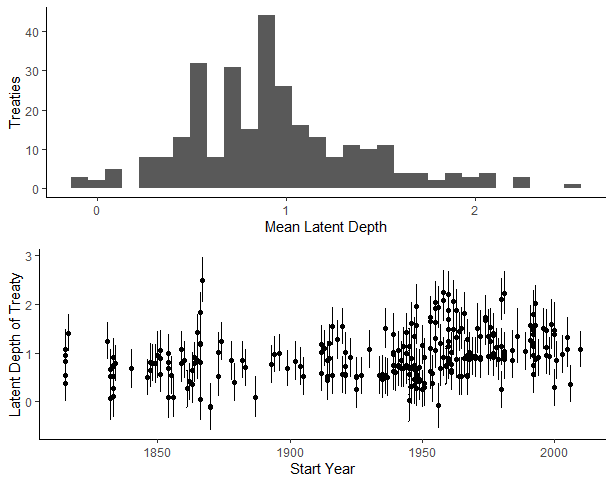
\includegraphics[width=0.95\textwidth]{../figures/ld-summary.png}
	\caption{Summary of the latent measure of alliance treaty depth for 289 defensive or offensive alliances from 1816 to 2016. The top panel plots the factor loadings with 90\% credible intervals. The bottom panel plots mean treaty depth (points) and the standard deviation (error bars) against the start year of the treaty.}
	\label{fig:ld-summary}
\end{figure}


% Cases- especially deep and shallow treaties
Although the values of the latent measure are not intrinsically meaningful and can therefore be positive or negative, differences between treaties on the latent scale are informative. 
The median of treaty depth is -0.09, and the mean is 0.05. 
The median treaty is the Southeast Asian Treaty Organization (SEATO), which includes a formal international organization (ATOP ID 3260). 
There are many shallow treaties that only include military support. 
One such alliance is an 1855 pact between France, the UK and Sweden (ATOPID 1190) which promises defense and consultation. 


Three of the deepest treaties are a 1993 alliance between Russia and Tajikistan (ATOPID 4470), a 1958 alliance between the UAE and Yemen (ATOPID 3345), and a 1981 pact between Gambia and Senegal (ATOPID 3930). 
All these alliances stipulate extensive defense cooperation. 
The alliance between Russia and Tajikistan includes military aid, bases, a companion military agreement, and integrated military command. 
The other two treaties attempted to establish a federation through military support, international organizations, basing, and defense policy coordination.


\begin{table}[hbt!]
\begin{center}
\begin{tabular}{cccc}
   Alliance  & Depth Score & Year & Depth Sources  \\
\hline
Brazil-Argentina-Uruguay & 1.01 & 1865 & Integrated Command, Military Aid, \\
                         &      &      &  Low Policy Coord., Subordination. \\
France-Russia   & .69 & 1893 & Moderate Policy Coord., Specific Contribution \\
 France-Poland   & -.75  & 1935  & None\\
 NATO & .32 & 1951 & Formal Organization, Basing rights \\ 
 Warsaw Pact & 1.2  & 1955 &  Formal IO, High Policy Coord., \\
             &      &      & Integrated Command  \\ 
\hline
\end{tabular}
\caption{Table of treaty depth estimates, year of formation and sources of depth for five alliances. }
\label{tab:depth-tab}
\end{center} 
\end{table}


\autoref{tab:depth-tab} provides five other examples of deep and shallow alliance treaty obbligations.  
The 1865 Triple Alliance between Brazil, Argentina and Uruguay included extensive cooperation for their war against Paraguay. 
An 1893 Franco-Russian alliance called for policy coordination and specified the number of troops each partner would provide in war. 
France's 1935 alliance with Poland has a minimal depth score, as it did not include any cooperation besides defensive and consultation obligations. 
As a result of ATOP's decision to omit the integrated command from formal treaty obligations, NATO scores above average on latent treaty depth, but it is not an overwhelmingly deep alliance in its formal treaty obligations.\footnote{Participation in the integrated command is not required by the NATO treaty, so ATOP does not count this as a treaty obligation. Basing rights are part of a 1951 additional protocol.}
Because the Warsaw Pact obligates members to join a formal organization, coordinate defense policy, and participate in an integrated command, it has greater formal depth than NATO. 
NATO has less depth because states like France and Greece could leave the integrated command structure without violating the alliance. 


The latent measure has some face, concept, and discriminant validity. 
As an example of face validity, the Gambia-Senegal federation requires deeper cooperation than arms-length commitments of military support. 
Shallow treaties promise little beyond military support, matching my conceptualization of treaty depth. 
Last, \autoref{fig:ld-summary} shows that this measure can distinguish between deep and shallow commitments. 


This latent treaty depth measure is the key explanatory variable in my empirical analysis. 
My argument claims that differences in depth among alliances modify the impact of alliance participation on percentage changes in military spending by alliance members at the state-year level of analysis. 
I use a multilevel model to capture this relationship, and summarize the estimation strategy in the next section. 


\subsection{Estimation: Multilevel Model} 


% Best fit for theoretical process. Can compare alliances. 
Because alliances and state-year observations are separate levels of analysis, I use a multilevel model to estimate the association between treaty depth and military spending and bridge the two data levels \citep{SteenbergenJones2002, GelmanHill2007}. 
My model estimates heterogeneous effects of alliance participation on military spending as a function of alliance characteristics, in order to make inferences about how alliance characteristics like formal depth modify the impact of individual alliances on military spending. 
To facilitate computation and interpretation, I fit the model using Bayesian estimation in STAN \citep{Carpenteretal2016}. 
See the appendix for details of the weakly informative prior distributions and evidence the chains converged.


This research design is more complicated than a panel data model like the estimator \citet{DigiuseppePoast2016} use, but the multilevel components add substantial value, especially by connecting the argument and research design.
I argue that treaty depth modifies the impact of alliance participation on growth in military spending. 
Differences in how alliance participation impacts military spending are the outcome of interest.  
The multilevel model explicitly compares the impact of participation in deep and shallow alliances by estimating how changes in treaty depth modify the consequences of alliance participation. 


Unlike the multilevel model, standard panel models employ state-level proxies for alliance characteristics, which compare states rather than alliances.
This practice of aggregating alliances at the state-year level of analysis may produce misleading inferences \citep[pg. 356]{McElreath2016}.
Summarizing alliance characteristics at a different level of analysis changes the mean and variance of key independent variables, which could affect inferences. 
Multilevel modeling avoids this aggregation problem by retaining the structure of alliance data, where states participate in multiple alliances and alliances could have heterogeneous effects on military spending.
The multilevel model estimates the specific impact of each alliance on members' military expenditures, thereby revealing differences between individual treaties. 
On the other hand, aggregating multiple alliances into state level indicators will mask any heterogeneous effects of individual treaties.\footnote{Partial pooling of the alliance-specific parameters generates reasonable estimates for each alliance.} 


Furthermore, multiple alliance characteristics affect the consequences of alliance participation.
The multilevel model captures multiple sources of heterogeneity in how alliances impact military spending. 
Treaty depth is correlated with other aspects of alliance membership and design, so this step is important.\footnote{For example, I show in another paper that democratic alliance membership is positively correlated with treaty depth.}
In a panel estimator with state-level proxies for alliance characteristics, accounting for correlated alliance characteristics is difficult. 
To account for several alliance characteristics, panel estimates must average different parts of a state's alliance portfolio or subset the data.
Averaging reduces theoretically interesting alliance-level variation, and analysis of multiple subsets risks generating spurious findings through multiple comparisons.  
In a multilevel model, I can account for how multiple alliance characteristics change the consequences of alliance participation by including other variables besides treaty depth in an alliance level regression. 
Therefore, my estimate of how treaty depth modifies the impact of alliance participation on military spending holds key alliance and state characteristics constant. 
I now describe the model specification in more detail. 
 


\subsubsection{Model Specification} 

% Two separate but connected regressions
% State-level regression- alliances enter through spending matrix.
This multilevel model connects two distinct regressions. 
The base is a state-year-level regression, which includes the impact of alliance participation.
A second alliance-level regression modifies the effect of alliance participation on military spending, like an interaction. 


The state-year-level regression starts with a distribution for the outcome:
\begin{equation}
y \sim student_t(\nu, \mu, \sigma)
\end{equation}
 

$y$ is the dependent variable--- percentage changes in military spending. 
I model the outcome using a t-distribution with degrees of freedom $\nu$ to address heavy tails and estimate $\nu$ directly.
$\sigma$ is analogous to the error term in a frequentist regression as it captures unexplained variation.  
$\mu$, the mean of the outcome, depends on several factors.
\begin{equation}
\mu = \alpha + \alpha^{st} + \alpha^{yr} +\textbf{W}_{n \times k} \gamma_{k \times 1}  + \textbf{Z}_{n \times a} \lambda_{a \times 1} 
\end{equation}


Percentage changes in spending are a function of an overall intercept $\alpha$, state and year varying intercepts $\alpha^{st}$ and $\alpha^{yr}$ and a matrix of state-level control variables $\textbf{W}$.
The $\textbf{Z} \lambda$ term incorporates alliance participation.
$\textbf{Z}$ is a matrix of state participation in alliances. 
Columns correspond to each of the $a$ alliances in the data, and rows to state-year observations. 
For this sample of non-major powers, $\textbf{Z}$ has 190 columns and 8,290 rows. 
If a state is not in a particular alliance, the corresponding matrix cell in that alliance column is zero.
If a state is part of the alliance in a given year, the matrix element contains the log of total allied military spending, which is normalized by year.\footnote{Normalization keeps the parameters on similar scales, which is important for modeling. The normalization is based of all 289 ATOP alliances, not just alliances with non-major powers.} %I selected normalization by the annual maximum theoretically and corroborated this choice by comparing models fit with different ways of expressing allied capability. See the appendix for details.} 
I use total allied spending to express the effect of alliance participation to match the theoretical emphasis on allied capability. 
$\textbf{Z}$ encodes a quasi-spatial indicator of alliance participation for all $a$ alliances in the data. 
States can be members of multiple treaties, so state-year observations are not neatly nested within alliances. 
This specification means each alliance has a unique impact on military spending, even when states participate in multiple treaties. 


$\lambda$ is a vector of parameters which estimate the impact of participation in specific alliances on military spending. 
Because the non-zero elements of $\textbf{Z}$ are allied spending, the $\lambda$ parameters capture alliance members' response to allied capability. 
Each alliance has a unique $\lambda$, so there are 190 alliance participation parameters. 
The $\lambda$ parameters have a shared distribution, so I assume alliances are similar but different in how they impact military spending. 


% Alliance-level regression:
The second part of the multilevel model uses alliance characteristics to predict how alliance participation is associated with percentage changes in military spending. 
The alliance participation parameters are the outcome in an alliance-level regression.
As a result, the impact of alliance participation on members' military spending depends on treaty characteristics, including depth. 
In this second-level regression: 


\begin{equation}
\lambda_{a} \sim N(\theta_{a}, \sigma_{all})
\end{equation} 
and 
\begin{equation}
\theta_{a} = \alpha_{all} + \beta_1 \mbox{treaty depth} + \textbf{X}_{a \times l} \beta
\end{equation}


% Like an interaction between alliance and state-level factors 
In the alliance-level regression, $\textbf{X}$ is a matrix of the $l$ alliance-level control variables and $\alpha_{all}$ is the constant.
Adding $\sigma_{all}$ means predictions of $\lambda$ are not deterministic--- the alliance level regression contains an error term. 
A larger $\sigma_{all}$ indicates more variation in how alliance participation impacts military spending. 


The second-level regression includes treaty depth, and each $\beta$ parameter modifies the impact of alliance participation on percentage changes in military spending. 
The $\beta$s are like marginal effects in an interaction. 
Treaty depth impacts military spending by modifying the consequences of alliance participation. 
Changing treaty depth shifts $\lambda$, which in turn affects military spending.
Hypothesis 3 predicts $\beta_1$ will be negative for non-major powers. 


In this model, the $\lambda$ parameters express heterogeneous effects of participation in individual alliances.
The $\beta$ parameters estimate how alliance characteristics modify the impact of alliance participation on military spending.  
Again, using alliance characteristics to predict the impact of alliance participation matches my conditional argument. 
I now describe the sample and key variables in the analysis.  



\subsection{Sample and Key Variables} 

% Sample of states & alliances: restricted to treaties with military support
I estimate the multilevel model on a sample of non-major power states from 1816 to 2007, including state-year observations with no alliances. 
I identify non-major powers using a measure of major power status from the Correlates of War Project. 
Alliance participation data comes from the ATOP project \citep{Leedsetal2002}.  
I focus on participation in defensive and offensive treaties, because prior studies of alliances and military spending examine these treaties. 
The sample contains data from 8,280 state-year observations and 190 alliances. 


% DV: percentage changes in milex
The dependent variable is percent changes in military spending, which is calculated as:
\begin{equation}
\mbox{\% Change Mil. Expend} = \frac{ \mbox{Change Mil. Expend}_t }{ \mbox{Mil. Expend}_{t-1} }
\end{equation} 
I used the Correlates of War Project's data on military spending to measure percentage changes in spending \citep{SingerCINC1988}.%\footnote{Estimating the model on SIPRI military spending data produces similar results: see the appendix for details.} 
The annual percentage change in spending equals that year's change in spending as a share of the previous year's military spending.
Thus, annual changes are bench marked to previous spending levels. 
To facilitate model fitting, I apply the inverse hyperbolic sine transformation to this variable.\footnote{This transformation applies to positive, negative and zero values. It has minimal impact on values between -1 and 1, but pulls in large positive values, which range as high as 140. Inferences about treaty depth and other alliance characteristics are comparable with and without the transformation.}
Using percentage changes in military expenditures as the dependent variable helps the research design. 
The level of military spending is not stationary for most states, especially in longer panels. 
Thus, using percentage changes in spending reduces the risk of spurious inferences.
Benchmarking changes to prior expenditures also facilitates comparisons across states and over time. 


% key IV: mean treaty depth
The key independent variable is the mean latent depth of each alliance, based on the measurement model. 
This variable enters the model in the alliance-level regression and I expect it will have a negative coefficient. 
I also include a series of state and alliance-level controls.


In the state-level regression, I adjust for several correlates of alliance participation and military spending. 
State-level covariates include GDP growth \citep{Boltetal2018} regime type, international war \citep{Reiteretal2016}, civil war participation \citep{SarkeesWayman2010}, annual MIDs \citep{Gibleretal2016}, rival military spending \citep{ThompsonDreyer2012} and a dummy for Cold War years.
Conflict participation, alliances, and military spending are all correlated \citep{SeneseVasquez2008}.
I include growth in GDP instead of levels because GDP levels are non-stationary and economic growth shapes the opportunity costs of military spending \citep{Kimball2010, Zielinskietal2017}.  

 
Other alliance level variables are correlates of treaty design and military spending, including the number of members and share of democracies in a treaty at time of formation \citep{Chibaetal2015}. 
I control for issue linkages by creating a dummy indicator of whether the alliance promises economic cooperation \citep{Poast2013, LongLeeds2006}. 
As an indicator of hierarchical security relationships, I include a count of foreign policy concessions in the alliance. 
I also mark the presence of unconditional military support using a dummy variable I constructed using existing indicators of conditional support in the ATOP data. 
Because threat may drive states to form deeper alliances and affect subsequent military spending, I control for the average threat of alliance members at the time of alliance formation using the threat measure of \citet{LeedsSavun2007}. 
I adjust for superpower membership--- whether the United States or Soviet Union participated in a treaty during the Cold War. 
Two dummy indicators of wartime alliances and asymmetric obligations \citep{Leedsetal2002} complete the alliance-level regression specification. 
Though I discuss these variables as controls, many of them are theoretically interesting in their own right. 
Having described the measure of treaty depth, multilevel model, and covariates, I now turn to the results of the analysis. 

 

\section{Results}


This section summarizes inferences from the multilevel model. 
I find support for all three hypotheses. 
Because shallow alliances tend to increase military spending and deep alliances often decrease spending, treaty depth and the effect of alliance participation on non-major power military spending are negatively correlated. 
Results are based on 2,000 samples from four chains, with 1,000 warm-up iterations. 
To facilitate model fitting, I employed a non-centered parameterization of the varying intercepts and a sparse matrix representation of \textbf{Z}. 
Standard convergence diagnostics indicate the chains adequately explored the posterior.\footnote{See the appendix for details on convergence and other robustness checks.} 


% note on interpreting Bayesian results
Because I used Bayesian modeling to estimate the association between treaty depth and percentage changes in military spending, each coefficient has a posterior distribution--- the likely parameter values conditional on the priors and observed data.
There are no indicators of statistical significance. 
Instead, I use the 90\% credible intervals of the parameters and calculate the negative posterior probability for the treaty depth coefficient to assess Hypothesis 3.\footnote{I use 90\% intervals because inferences about 95\% intervals are sensitive to simulation variance in Bayesian analysis.}


\autoref{fig:results-allreg} summarizes the coefficient estimates from the alliance-level regression and the simulated substantive effect of greater treaty depth. 
The preponderance of evidence matches Hypothesis 3, as shown in the top panel of \autoref{fig:results-allreg}.
There is a 96\% chance treaty depth is negatively correlated with the impact of alliance participation on percent changes in military spending for non-major powers.
As treaty depth rises, the effect of alliance participation on military spending falls. 


\begin{figure}[htbp]
	\centering
		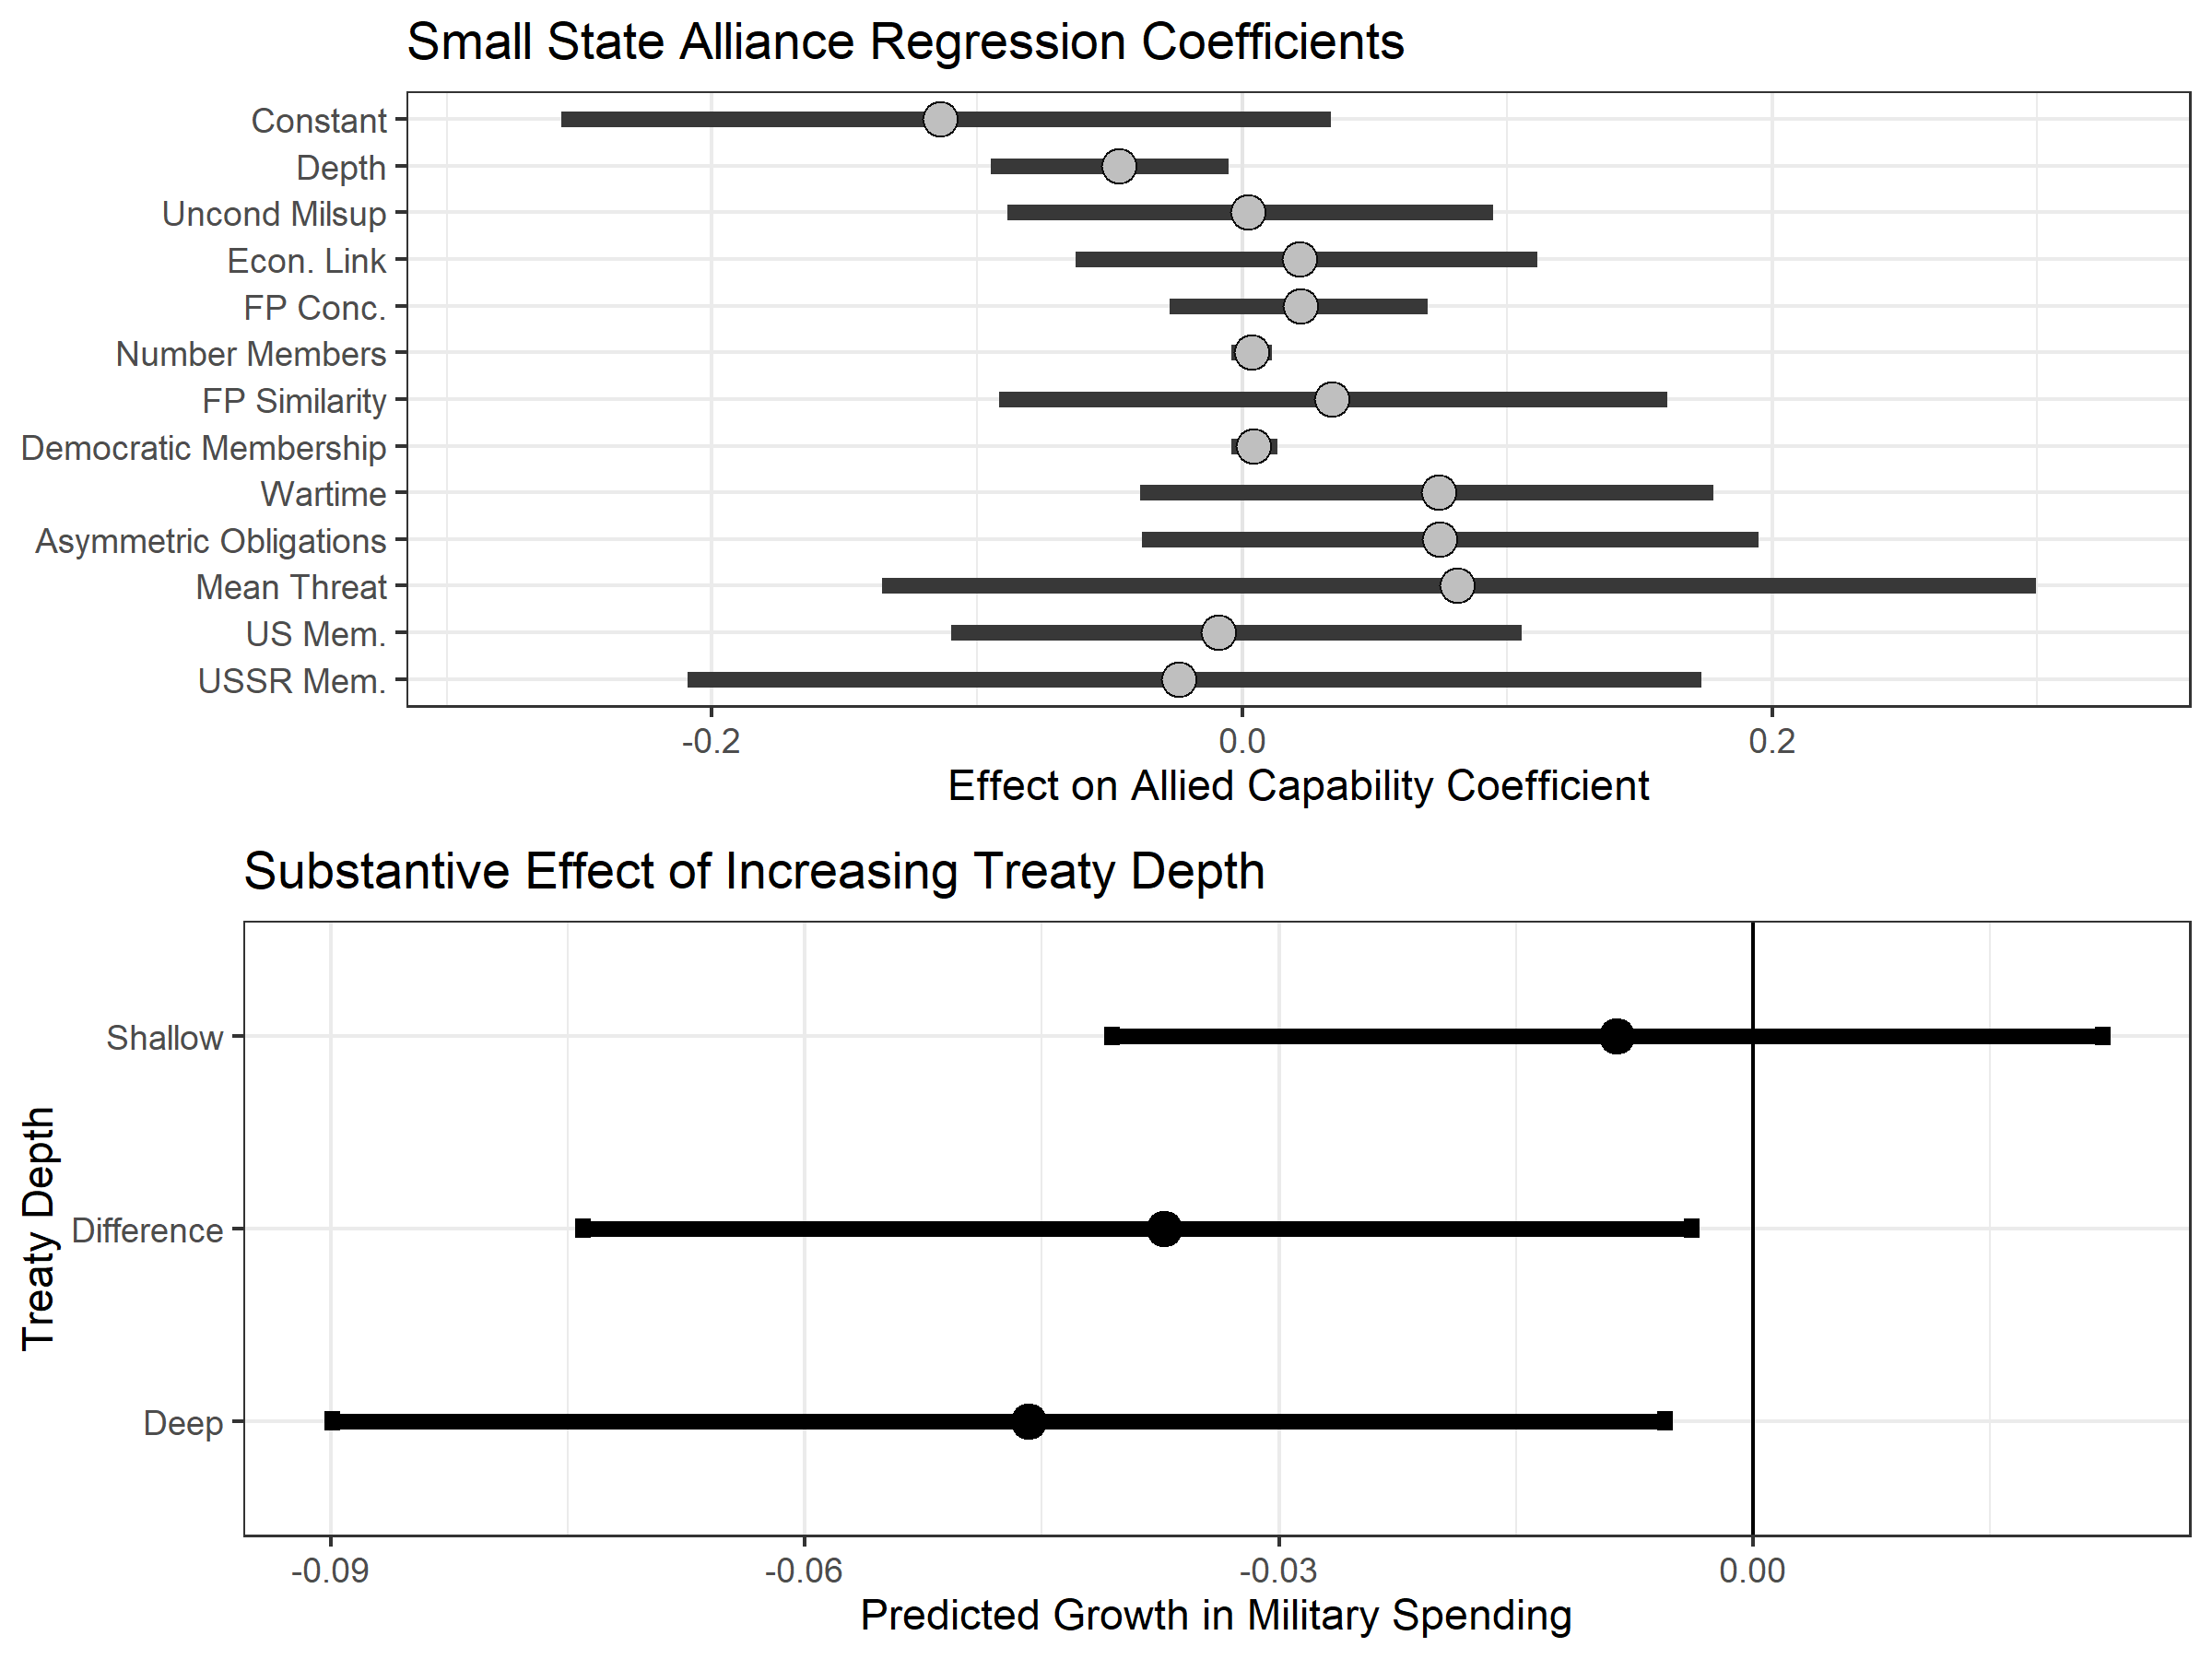
\includegraphics[width=0.95\textwidth]{../figures/results-allreg.png}
	\caption{Summary of alliance-level regression results from the multilevel model of alliance participation and military spending. The top panel shows the 90\% credible intervals for coefficients in the alliance-level regression. The bottom panel plots the estimated effect of participation in an alliance with average capability on growth in military spending for a deep and shallow treaty, as well as the difference between deep and shallow alliances. In both panels, points mark the posterior mean, and the bars encapsulate the width of the 90\% credible interval.}
	\label{fig:results-allreg}
\end{figure}


I plot the substantive effect of the alliance-level depth coefficient in the bottom panel of \autoref{fig:results-allreg}. 
I assess this substantive effect by simulating the effect of changing treaty depth from the minimum value of -0.8 to 1.5. 
Holding other alliance covariates at their modes or medians, this increase in depth reduces a hypothetical alliance parameter $\lambda$ by .08 in expectation, which then lowers military spending growth.
The results of the the simulation are summarized by 90\% intervals for predicted growth in military spending in the hypothetical shallow alliance, predicted spending growth in the hypothetical deep alliance, and the difference between those two scenarios.
Assuming the hypothetical alliance has median capability, the difference in spending growth between the shallow and deep treaty has a mean of -.03.
The 90\% credible interval of this predicted fall in military spending due to increasing treaty depth ranges from -0.056 to -0.001.
Although the range of estimated substantive effects includes small values, there is a perceptible difference between non-major power military spending growth in deep and shallow alliances, all else equal.  


To assess Hypotheses 1 and 2, I examine patterns in the alliance participation parameters across the range of treaty depth.
Each $\lambda$ measures the impact of treaty participation, so if treaty depth has a large influence on alliance participation, it will appear in the $\lambda$ estimates. 
On average, participation in deep alliances should have a negative effect on members' percent changes in military spending and shallow alliances should have a positive effect.
If this is true, there will also be a negative trend in the expected value of $\lambda$ as treaty depth increases.


\begin{figure}[htbp]
	\centering
		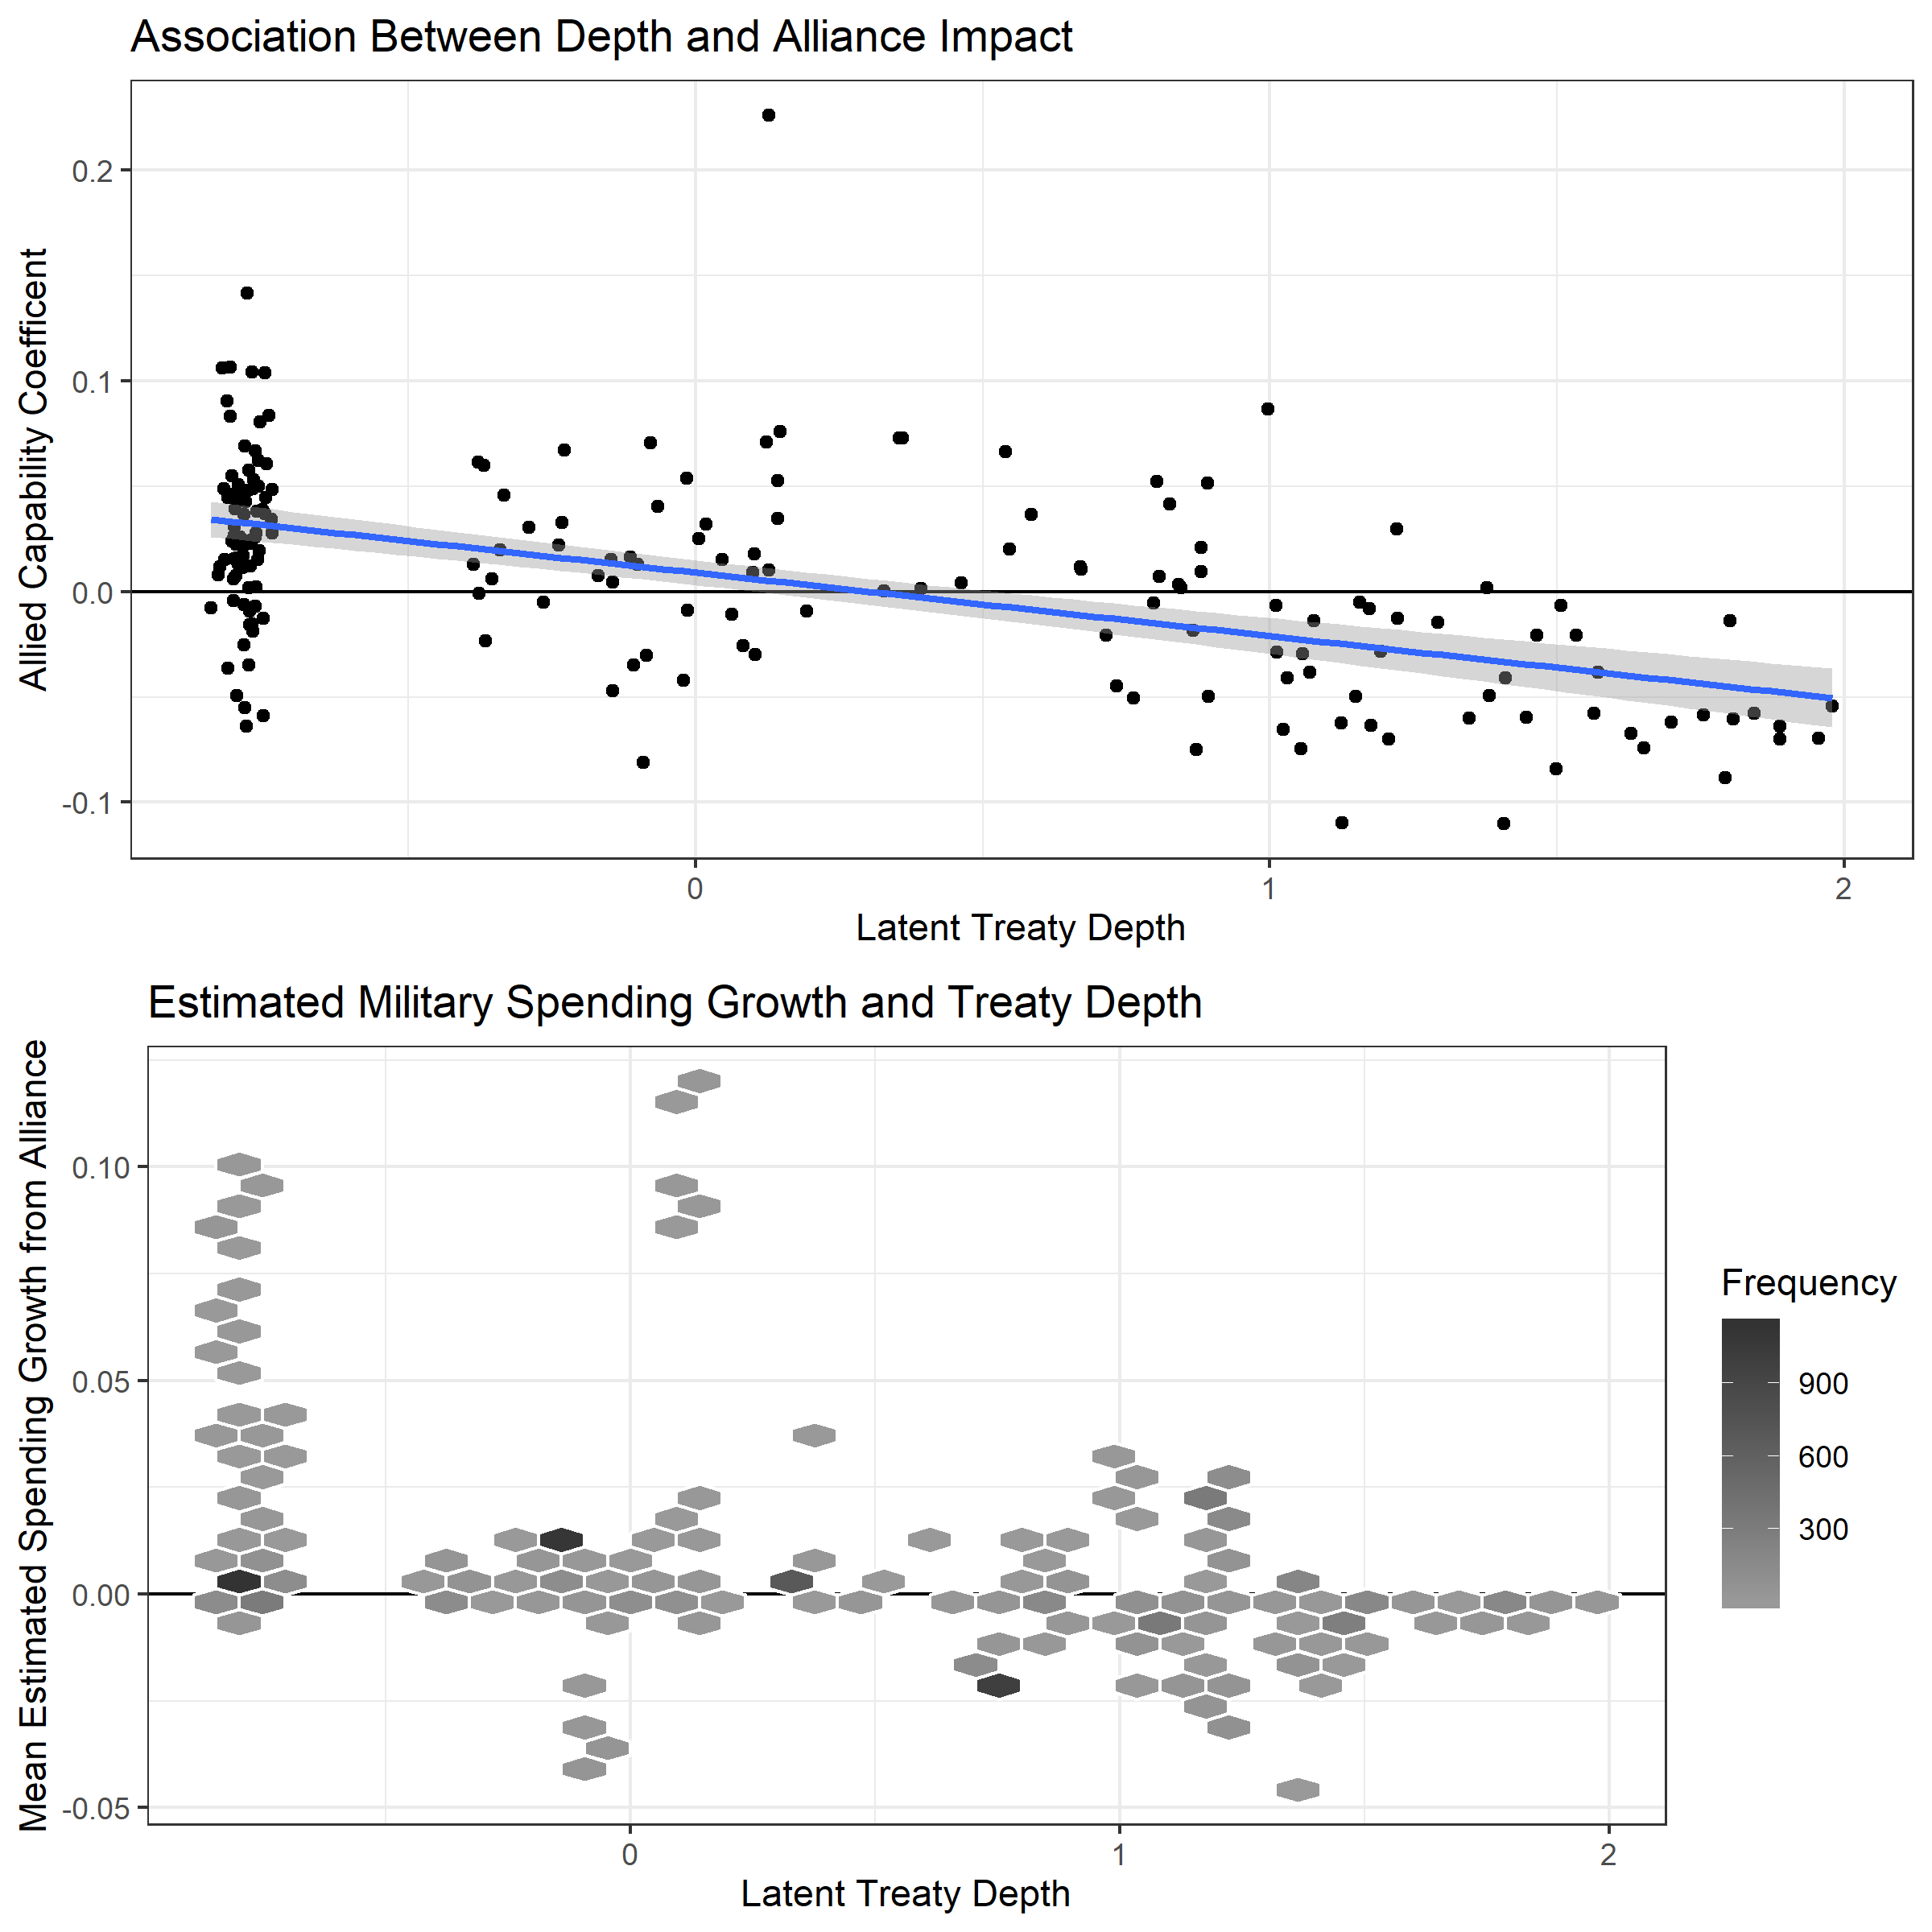
\includegraphics[width=0.95\textwidth]{../figures/results-allpred.png}
	\caption{Summary of the predicted effect of alliance participation on growth in military spending across the observed values of treaty depth for 190 alliances from 1816 to 2007. The top panel plots the mean of each $\lambda$ parameter by treaty depth. The bottom panel plots 9,128 state-alliance-year estimates of how participation in individual alliances affects growth in military spending, which are the product of the $\lambda$ for the alliance and allied capability value for that state-year observation. Darker shading indicates more data points in the hexagon.}
	\label{fig:results-allpred}
\end{figure}


The preponderance of evidence in \autoref{fig:results-allpred} matches the predictions of Hypotheses 1 and 2.
The top panel of \autoref{fig:results-allpred} plots the expected value of the alliance participation parameter across the range of treaty depth. 
As expected, shallow treaties often have positive $\lambda$ values,\footnote{All the negative $\lambda$ estimates in alliances with minimal depth are treaties between the Soviet Union and Eastern European states during the Cold War.} which corresponds to Hypothesis 1. 
Most of the deepest treaties have a negative $\lambda$, which matches Hypothesis 2. 
Because other treaty characteristics and chance also influence the $\lambda$ estimates, there is substantial variation in how alliance participation impacts non-major power military spending. 


I then used the $\lambda$ posteriors to estimate the impact of alliance participation on state-year military spending growth. 
To assess the annual impact of alliances on their members, I multiplied the alliance membership matrix $\textbf{Z}$ by the $\lambda$ parameters to generate 9,124 non-zero state-alliance-year predictions.\footnote{These estimates hold all state-level variables constant.} 
The scatter plot in the bottom panel of \autoref{fig:results-allpred} shows the distribution of predicted changes in military spending from alliance participation.
Each point marks the mean estimated effect of an alliance on growth in military spending for that state-year.
To avoid overplotting the 9,124 point estimates, I combined them into hexagons. 
Darker hexagons mark areas with more points. 
As Hypothesis 1 predicts, participation in shallow alliances regularly increases military spending. 
Many alliances with shallow depth have little effect on military spending, however. 
As treaty depth increases, alliance participation is more likely to reduce military spending growth.\footnote{Wartime alliances are the main exception to this trend.}
Some of the deepest alliances have a negligible effect on military spending despite negative $\lambda$ values due to limited capability. 


The appendix contains a series of robustness checks for this specification.
First, I fit models with the three-level ordinal measure of \citep{LeedsAnac2005}, and find that their military institutionalization measure also reduces the impact of alliance participation on non-major power military spending. 
I also fit a model that shifted the distribution of latent depth to include only zero and positive values. 
Last, I include single level panel regressions that average or summarize states' alliance portfolio in several ways. 


In summary, I find that treaty depth modifies the impact of alliance participation on military spending.  
Participating in deep alliances often reduces military spending, while being part of a shallow alliance often increases spending. 
I now discuss the implications of the argument and results. 



\section{Discussion and Conclusion}


% Precise interpretation: compares alliances. Not treaty vs absence. 
This paper addresses a longstanding debate over whether alliance participation increases or decreases military spending. 
Claims alliance participation only increases or decreases military spending are incomplete. 
My argument shows how treaty depth modifies the impact of alliance participation on military spending, which builds on other conditional arguments \citep{DigiuseppePoast2016}. 
I show that whether alliance participation increases or decreases military spending depends on treaty depth. 
Compared to no alliance at all, joining a shallow treaty usually increases military expenditures, while participation in a deep alliance often lowers defense spending. 


% two results that are new & maybe puzzling
There are two other noteworthy findings.  
First, many alliances increase non-major power military spending, which cuts against expectations that non-major powers are inveterate free-riders. 
To gain security from alliance participation, non-major powers sometimes need to increase their defense budget \citep{Horowitzetal2017}. 
Second, the military spending growth predictions in \autoref{fig:results-allpred} suggest that many alliances have little effect on military spending, which is puzzling given widespread expectations that alliances and military spending are related. 
These negligible effects could reflect offsetting effects from different parts of alliance treaty design and membership, or concerns about the credibility of many alliance treaties. 


Given my departure from previous research designs, how should we compare these results to prior evidence on alliance participation and military spending? 
Connecting my results with earlier evidence requires renewed attention to specific and general research designs. 
Recall that general studies compare states in an alliance to those without one in a global sample and specific studies estimate responses to allied military spending in a few alliances. 
The results encompass specific and general research designs by using allied capability to measure alliance participation. 
Each alliance participation parameter includes the effect of joining an alliance and changes in allied capability. 
I then use the alliance-level regression to understand how the impact of alliance participation varies with treaty design and membership.   


Although my research design advances the debate on alliance participation and military spending, it has two limitations. 
First, my findings only address formal treaty depth. 
The measure of treaty depth only includes formal promises, in part because informal depth is harder to observe. 
As a result, my test of alliance depth may be conservative--- it does not capture phenomena that should have a similar effect. 
It could instead overstate the findings if formal depth is not implemented, however. 
Strategic alliance design is the second possible weakness of the test. 
Domestic politics can affect alliance obligations, for example \citep{Davis2004, Chibaetal2015}.   
To address this issue, I controlled for correlates of alliance participation and treaty depth at each level of the model, with a particular focus on factors like democracy, alliance size, external threat, and other sources of credibility.
At the state level, I adjusted for threat, economic growth, and regime type, all of which are possible correlates of treaty depth and growth in military spending. 
Even with this effort, selection into different alliances could still produce unobserved differences between alliances I did not adjust for. 


Despite these limitations, the argument and results generate valuable insights about alliance participation and military spending. 
I explain when alliance participation is associated with increases or decreases in military spending among non-major powers, which addresses a debate between contradictory views of alliances.  
I provide evidence that how alliance participation impacts military spending depends on state capability and alliance treaty depth using a new measure of alliance treaty depth and a multilevel model. 


% Concluding implications: scholarship 
There are several implications for scholarship. 
First, my argument and findings reinforce the importance of accounting for heterogeneity among alliances and institutional design more generally.
Second, my research design could apply to other international institutions where institutional design shapes the consequences of participation.
Besides these general implications, the results raise interesting questions for future research. 
For example, why do many alliances have a negligible effect on non-major power military spending? 
Because arms and alliances both provide security, existing arguments expect they are connected, but I find that many alliances have little substantive effect.
The domestic economic and political consequences of alliance participation also remain relatively unexplored.
Research on this topic could explore how changes in allied military spending affect public support for alliance participation and the economic consequences of changes in military spending.  


% The argument indicates tradeoff: set up policy implication
Besides their scholarly value, the argument and evidence help inform policy debates about military spending. 
My argument claims that reassurance from deep alliances leads to lower defense spending. 
States can use deep cooperation to increase alliance credibility, but allied military spending may fall in response. 
Therefore, there is a tradeoff between treaty credibility and allied military spending. 


% Implications for policy. 
The United States is currently wrestling with the credibility-military spending tradeoff. 
Washington has often decried allies who provide too little for their own defense \citep{Lanoszka2015}. 
But allies are able to maintain low military spending partly because the United States makes deep commitments. 
Reducing the depth of US alliances could generate credibility problems, however. 
Low allied defense spending may be the price of credible commitments.  
Therefore, this paper is not an unconditional call to reduce the depth of US alliances. 
Adjusting existing treaties may be more difficult than designing new alliances and could have other ramifications. 
The full consequences of shifting treaty depth require additional scrutiny. 

 



\singlespace
 
\bibliography{../../MasterBibliography} 





\end{document}
